\documentclass[11pt]{article}
\usepackage[T1]{fontenc}
\usepackage{lmodern}
\usepackage[sc]{mathpazo}
\usepackage{amsmath,amssymb,amsthm,mathtools}
\usepackage{microtype}
\usepackage[letterpaper,top=0.85in,bottom=0.87in,left=0.95in,right=0.95in,headheight=15pt,headsep=19pt]{geometry}
\usepackage{booktabs,array,tabularx,enumitem}
\usepackage{xcolor,tikz,titlesec,fancyhdr,listings}
\usetikzlibrary{arrows.meta,calc,positioning,decorations.pathreplacing}
\definecolor{ink}{HTML}{173B4D}
\definecolor{teal}{HTML}{277D79}
\definecolor{gold}{HTML}{B58B4A}
\definecolor{slate}{HTML}{5A6971}
\definecolor{mist}{HTML}{EEF4F4}
\usepackage[colorlinks=true,linkcolor=ink,citecolor=teal,urlcolor=teal,breaklinks=true]{hyperref}
\usepackage[nameinlink,noabbrev]{cleveref}
\crefname{theorem}{Theorem}{Theorems}
\crefname{lemma}{Lemma}{Lemmas}
\crefname{proposition}{Proposition}{Propositions}
\crefname{corollary}{Corollary}{Corollaries}
\crefname{definition}{Definition}{Definitions}
\crefname{section}{Section}{Sections}
\crefname{figure}{Figure}{Figures}
\crefname{table}{Table}{Tables}
\hypersetup{pdfauthor={John Tripodo},pdftitle={Separated distances in fixed dimension},pdfsubject={Two-circle tolerance family and a dimension-29 counterexample}}
\numberwithin{equation}{section}
\newtheorem{theorem}{Theorem}[section]
\newtheorem{proposition}[theorem]{Proposition}
\newtheorem{lemma}[theorem]{Lemma}
\newtheorem{corollary}[theorem]{Corollary}
\theoremstyle{definition}\newtheorem{definition}[theorem]{Definition}
\theoremstyle{remark}\newtheorem{remark}[theorem]{Remark}
\newcommand{\R}{\mathbb R}\newcommand{\N}{\mathbb N}
\newcommand{\ip}[2]{\langle #1,#2\rangle}
\newcommand{\norm}[1]{\lVert #1\rVert}
\newcommand{\opnorm}[1]{\lVert #1\rVert_{\mathrm{op}}}
\newcommand{\T}{\mathsf T}\newcommand{\one}{\mathbf1}
\newcommand{\code}[1]{{\ttfamily\small #1}}
\newcommand{\TripodoCommit}{\texttt{1e73a12}}
\DeclareMathOperator{\diam}{diam}\DeclareMathOperator{\diag}{diag}
\titleformat{\section}{\Large\bfseries\color{ink}}{\thesection}{.7em}{}
\titleformat{\subsection}{\normalsize\bfseries\color{ink}}{\thesubsection}{.65em}{}
\titlespacing*{\section}{0pt}{22pt}{10pt}
\titlespacing*{\subsection}{0pt}{16pt}{6pt}
\setlength{\parindent}{1.15em}
\setlength{\parskip}{2pt}
\setlength{\tabcolsep}{5pt}
\renewcommand{\arraystretch}{1.12}
\linespread{1.055}
\emergencystretch=2em
\setlength{\abovecaptionskip}{7pt}
\setlength{\belowcaptionskip}{5pt}
\pagestyle{fancy}\fancyhf{}
\fancyhead[L]{\scriptsize\scshape\color{slate}Separated distances in fixed dimension}
\fancyhead[R]{\scriptsize\color{slate}John Tripodo}
\fancyfoot[L]{\scriptsize\color{slate}20 October 2026}
\fancyfoot[R]{\small\color{ink}\thepage}
\renewcommand{\headrulewidth}{0.3pt}
\renewcommand{\footrulewidth}{0pt}
\lstset{basicstyle=\ttfamily\scriptsize,keywordstyle=\color{ink}\bfseries,commentstyle=\color{slate},stringstyle=\color{teal},breaklines=true,columns=fullflexible,keepspaces=true,showstringspaces=false,frame=single,rulecolor=\color{teal!35},backgroundcolor=\color{mist},xleftmargin=5pt,xrightmargin=5pt,aboveskip=10pt,belowskip=10pt}
\begin{document}
\thispagestyle{fancy}
\noindent{\sffamily\small\bfseries\color{teal}METRIC GEOMETRY\quad /\quad ERD\H{O}S PROBLEM 670}\par
\vspace{18pt}
\noindent{\fontsize{30}{34}\selectfont\bfseries\color{ink}Separated distances\\[3pt]in fixed dimension}\par
\vspace{10pt}
\noindent{\Large\color{slate}Two circles and a\\[2pt]dimension-29 counterexample}\par
\vspace{15pt}
\noindent{\large John Tripodo}\hfill{\small 20 October 2026}\par
\vspace{3pt}
\noindent{\small\color{slate}\href{https://orcid.org/0009-0006-9180-4953}{ORCID 0009-0006-9180-4953}}\par
\vspace{13pt}\noindent{\color{gold}\rule{\textwidth}{1pt}}\par
\vspace{8pt}
\noindent\textbf{Abstract.}
A finite Euclidean point set is distance-separated when the lengths of any
two different unordered edges differ by at least one. The counting bound
for its diameter is asymptotically $n^2/2$, whereas Erd\H{o}s asked for a
coefficient-one lower bound. We give a two-circle construction: for every
$0<\varepsilon\le1/2$ and every $n\ge4\lceil8192/\varepsilon\rceil$, there
is a distance-separated $n$-point set in
$\R^{10\lceil8192/\varepsilon\rceil-1}$ with diameter
$<(1/2+\varepsilon)n^2$. A uniform form has coefficient
$1/2+102400/d+40960/n$. Independently, an explicit six-vertex macro seed
gives arbitrarily large configurations in the single space $\R^{29}$
with diameter $<0.998n^2$, refuting the maintained fixed-dimensional
coefficient-one statement. A short-prime-interval theorem also gives
diameter $<0.999n^2$ in $\R^{29}$ for every $n\ge400000$. Two orthogonal circle channels separate local
ruler gaps from cross-edge digits; the latter have an exact monotone
square-root formula. The small-dimensional proof uses three rational
matrix certificates valid for all admissible finite cluster sizes.
The two-circle family and the prime-first dimension-29 theorem have
corresponding Lean~4 proofs; the all-size corollary is a written consequence. The general family
uses uniform colex estimates; the dimension-29 construction replaces them
with a finite rational certificate.
\vspace{12pt}
\begin{center}
\fcolorbox{teal!30}{mist}{\parbox{.92\textwidth}{\small\color{ink}
\textbf{GitHub manuscript, 20 October 2026.}
The prime-first theorem and its all-size corollary have different bounds
and verification scopes. The near-counting family fixes the dimension
separately for each tolerance.}}
\end{center}
\vspace{5pt}
\noindent{\footnotesize\textbf{Keywords:} separated distances, Euclidean diameter,
Gram completion, quadratic-residue rulers, Lean formalization.}
\clearpage

\section{The problem and the results}\label{sec:intro}

How small can the diameter of a point configuration be if all of its edge
lengths must stay at least one unit apart? The number of edges gives a
quadratic lower bound. In a fixed Euclidean dimension, however, the geometry
may impose a further loss. This paper gives two constructions that separate
these questions: a uniform family approaching the counting coefficient as
the dimension increases, and a counterexample to the coefficient-one bound
in dimension~29.

\begin{definition}
An \emph{edge} of a finite set $X\subset\R^d$ is an unordered pair of distinct
points. We call $X$ \emph{distance-separated} if
\begin{equation}\label{eq:separated}
 \bigl|\norm{x-y}-\norm{u-v}\bigr|\ge1
 \quad\text{for any two different edges }\{x,y\},\{u,v\}.
\end{equation}
For $n\ge3$, let $\Delta_d(n)$ be the infimum of the diameters of all
distance-separated $n$-point subsets of $\R^d$.
\end{definition}

The comparison in \eqref{eq:separated} is between edges, not merely between
distinct values in a distance set: repeated edge lengths are forbidden.
Every edge has length at least one. Indeed, if $z$ is a third point, then
$1\le|\norm{x-z}-\norm{y-z}|\le\norm{x-y}$. Sorting the $\binom n2$ edge
lengths therefore gives
\begin{equation}\label{eq:counting}
 \Delta_d(n)\ge\binom n2=\left(\frac12-o(1)\right)n^2.
\end{equation}
The class defining the infimum is nonempty: the positive differences between
distinct powers of two are distinct integers, so a suitable set on a line
already supplies an example.

Erd\H{o}s asked whether the stronger lower bound $(1+o(1))n^2$ holds;
see \cite[Problem~20]{Erdos}. His wording does not specify the quantifier
order in the dimension. The maintained fixed-dimensional interpretation is
\begin{equation}\label{eq:conjecture}
 \forall d\ge1\ \forall\varepsilon>0\ \exists N\ \forall n\ge N:
 \quad \Delta_d(n)\ge(1-\varepsilon)n^2.
\end{equation}
The threshold $N$ may depend on both $d$ and $\varepsilon$.

Ho's earlier construction \cite{Ho} refutes a bound uniform in dimension:
for infinitely many $n$, it gives configurations in $\R^{n^2-n}$ with
diameter $(1-1/\pi^2+o(1))n^2$. His Remark~10 proves the improved coefficient
$(\pi+\sqrt{\pi^2-4})/(2\pi)=0.885589\ldots$ in that construction, while
Remark~9 leaves the fixed-dimensional question open. His proof also has a
Lean formalization. The distinction addressed here is the dimension's
independence from the number of points.

The earlier unrestricted-dimensional construction \cite{GrowingDimension}
achieves diameter $\binom n2+O(\sqrt{\log n})$ for every $n\ge3$, with
dimension allowed to grow with $n$. Here the aim is to keep the dimension
fixed while the number of points grows.

\subsection{Dimension linear in the inverse tolerance}

\begin{theorem}[The two-circle family]\label{thm:epsilon}
Let $0<\varepsilon\le\tfrac12$ and put
$m_0=\lceil8192/\varepsilon\rceil$. For every integer $n\ge4m_0$ there is an
$n$-point set $X\subset\R^{10m_0-1}$ with minimum point
distance at least one, with the lengths of different unordered edges
\emph{strictly} more than one apart, and with
\[
 \diam X<\left(\frac12+\varepsilon\right)n^2.
\]
\end{theorem}

For each fixed tolerance, both the ambient dimension and the size threshold
are $O(\varepsilon^{-1})$. The same construction gives a useful statement
when dimension and point count are specified in advance.

\begin{corollary}[Uniform dimension and size]\label[corollary]{cor:uniform}
If $d\ge163840$ and $n\ge65536$, there is a configuration in $\R^d$ with the
same minimum-distance and strict edge-separation properties and
\[
 \diam X<\left(\frac12+\frac{102400}{d}+\frac{40960}{n}\right)n^2.
\]
\end{corollary}

The dimension depends on $\varepsilon$ in \cref{thm:epsilon}. Consequently,
neither statement constructs diameter $(1/2+o(1))n^2$ in one fixed dimension.
The $O(1/d+1/n)$ order was already present in the earlier internal
deterministic-incidence construction~\cite{IncidenceNote}; the contribution of the present
organization is a simpler two-circle proof with explicit constants, together
with its exact formal endpoint. No optimality of this dimension order is
asserted.

\subsection{A fixed witness in dimension 29}

\begin{theorem}[Dimension 29]\label{thm:r29}
For every natural number $N$, there exist an integer
$n\ge\max\{N,600\}$ and a set $X\subset\R^{29}$
of $n$ points such that the minimum point distance is at least one, different
unordered edge lengths differ by at least one, and
\[
 \diam X<\frac{499}{500}n^2=0.998n^2.
\]
The sizes arise along an unbounded prime-first subsequence.
\end{theorem}

\begin{corollary}[All sufficiently large sizes in dimension 29]\label[corollary]{cor:r29-all}
For every integer $n\ge400000$, there is an $n$-point set in $\R^{29}$
with minimum point distance at least one, distinct unordered edge lengths
strictly more than one apart, and diameter $<0.999n^2$.
\end{corollary}
This corollary uses an explicit prime-interval theorem in addition to the
same geometry. Its written proof is given at the end of
\cref{sec:r29-proof}; it is not one of the Lean endpoints listed in
\cref{sec:formal}.

\begin{corollary}[Negation of the fixed-dimensional statement]\label[corollary]{cor:negation}
The proposition \eqref{eq:conjecture} is false. In fact,
$\liminf_{n\to\infty}\Delta_{29}(n)/n^2\le499/500<1$.
\end{corollary}
\begin{proof}
If \eqref{eq:conjecture} held, choose $d=29$ and $\varepsilon=1/1000$.
Its eventual lower bound $0.999n^2$ contradicts \cref{thm:r29} at a selected
size beyond that threshold.
\end{proof}

The dimension-29 theorem trades a weaker diameter coefficient for a much
smaller dimension and different size quantifiers. The earlier published
orthogonal-circle theorem \cite{PublishedFinite} gives diameter below
$0.735n^2$ in $\R^{81794}$ for \emph{every} $n\ge36354$. That theorem remains
valid; it is not superseded in every parameter by \cref{thm:r29}.

\begin{table}[ht]
\centering\small
\begin{tabularx}{\textwidth}{@{}p{.23\textwidth}p{.24\textwidth}X@{}}
\toprule
Construction & Ambient dimension & Diameter and size quantifier\\
\midrule
Published finite version & $81794$ & $<0.735n^2$ for every $n\ge36354$\\[4pt]
\Cref{thm:r29} & $29$ & $<0.998n^2$ for arbitrarily large selected $n\ge600$\\[4pt]
\Cref{cor:r29-all} & $29$ & $<0.999n^2$ for every $n\ge400000$ (written corollary)\\[4pt]
\Cref{thm:epsilon} & $10\lceil8192/\varepsilon\rceil-1$ &
$<(1/2+\varepsilon)n^2$ for every $n\ge4\lceil8192/\varepsilon\rceil$\\
\bottomrule
\end{tabularx}
\caption{The results have different quantifiers. The dimension in the last
row is fixed for each chosen tolerance, independently of $n$.}
\label{tab:results}
\end{table}

\subsection{Why two circles help}

Replace each of $m$ macro vertices by $k$ points. Distances within a cluster
must all be distinct, while each pair of clusters contributes an ordered
block of $k^2$ cross lengths. A tilted circle can encode the coarse and fine
digits of those blocks. A second circle, in independent coordinates, can
encode the local ruler without constraining its angular span to the digit
circle's small arc. A whole-matrix Gram completion makes the perturbation
spaces of different clusters orthogonal. The resulting cross lengths are
\emph{exactly}
\[
 \Phi_\nu(T)=\sqrt{\nu^2+2\nu T}.
\]
This formula requires only a derivative bound. Its error relative to
$\nu+T$ need not remain bounded as the clusters grow.

\begin{figure}[ht]
\centering
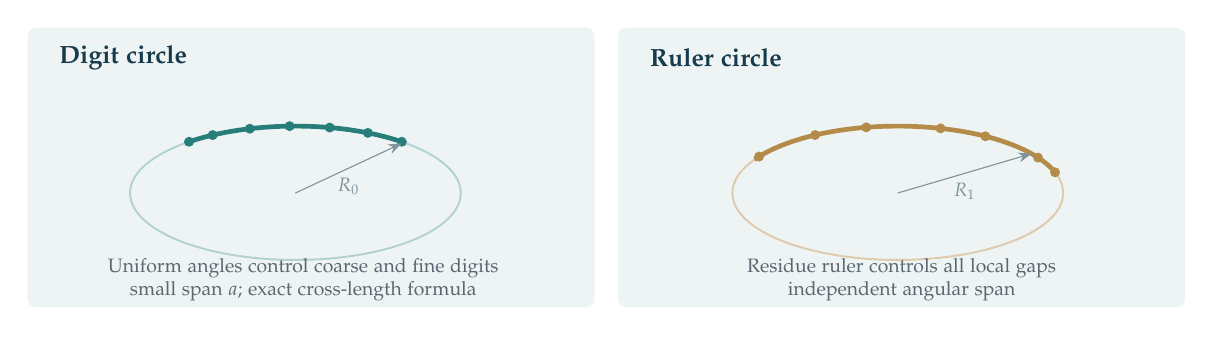
\begin{tikzpicture}[x=1cm,y=1cm,>=Stealth,font=\small]
\fill[mist,rounded corners=3pt] (0,0) rectangle (7.2,3.55);
\fill[mist,rounded corners=3pt] (7.5,0) rectangle (14.7,3.55);
\node[anchor=west,font=\small\bfseries,text=ink] at (.28,3.17) {Digit circle};
\node[anchor=west,font=\small\bfseries,text=ink] at (7.78,3.17) {Ruler circle};
\draw[teal!35,line width=.7pt] (3.4,1.45) ellipse (2.1 and .85);
\draw[teal,line width=1.7pt] plot[domain=48:132,samples=70] ({3.4+2.1*cos(\x)},{1.45+.85*sin(\x)});
\foreach \a in {50,64,78,92,106,120,130} {\fill[teal] ({3.4+2.1*cos(\a)},{1.45+.85*sin(\a)}) circle(1.8pt);}
\draw[ink!55,->] (3.4,1.45)--(4.75,2.08) node[midway,below,font=\scriptsize] {$R_0$};
\node[font=\scriptsize,align=center,text=slate] at (3.5,.35) {Uniform angles control coarse and fine digits\\small span $a$; exact cross-length formula};
\draw[gold!45,line width=.7pt] (11.05,1.45) ellipse (2.1 and .85);
\draw[gold,line width=1.7pt] plot[domain=15:150,samples=70] ({11.05+2.1*cos(\x)},{1.45+.85*sin(\x)});
\foreach \a in {18,32,58,75,101,120,147} {\fill[gold] ({11.05+2.1*cos(\a)},{1.45+.85*sin(\a)}) circle(1.8pt);}
\draw[ink!55,->] (11.05,1.45)--(12.75,1.95) node[midway,below,font=\scriptsize] {$R_1$};
\node[font=\scriptsize,align=center,text=slate] at (11.1,.35) {Residue ruler controls all local gaps\\independent angular span};
\end{tikzpicture}
\caption{Two independent coordinate channels within each cluster, shown
schematically. The ellipses depict circle planes; they are not a literal
planar realization of the high-dimensional construction. Whole-matrix
completion makes different clusters' perturbation spaces orthogonal.}
\label{fig:architecture}
\end{figure}


The general family uses a colex-labelled macro simplex with uniform
operator estimates. The dimension-29 construction replaces that large
simplex by six vertices with an explicit label pattern. Three exact
$5\times5$ positivity checks then control \emph{all} cluster sizes in its
admissible range. The proofs below retain these two distinct macro inputs.

The common geometry and separation lemmas are proved in
\cref{sec:mechanism}. The general family uses the colex input from
\cref{sec:macro}; its proof, including the passage to every sufficiently
large size, is in \cref{sec:epsilon-proof}. The dimension-29 proof in
\cref{sec:r29-proof} replaces the macro input and numerical parameters.

\section{The common geometric mechanism}\label{sec:mechanism}

We use real Euclidean inner products, transpose $\T$, and the operator norm
$\opnorm{\cdot}$. Matrices act on column vectors. For a prime $p$, write
$[v]_p\in\{0,\ldots,p-1\}$ for the least nonnegative residue.

\begin{lemma}[Two-circle completion]\label[lemma]{lem:completion}
Let $R_0,R_1>0$, let $q_A\in\R^{m-1}$, $0\le A<m$, and let $U$ be an $(m-1)\times m$ matrix
with $\opnorm U\le R_0$. Put
$W=(R_0^2I-U^\T U)^{1/2}$. For real $z,w$, define
\begin{align*}
 \eta_A(z)&=(U_A\sin z,\,We_A\sin z,\,R_0e_A\cos z),\\
 \zeta_A(w)&=(R_1e_A\sin w,\,R_1e_A\cos w).
\end{align*}
The vector $\eta_A(z)$ lies in $\R^{m-1}\oplus\R^m\oplus\R^m$ and has norm
$R_0$; $\zeta_A(w)$ lies in two further $m$-dimensional blocks and has norm
$R_1$. The perturbation spaces for different $A$ are orthogonal. Within one
cluster the two chord lengths are respectively
$2R_0|\sin((z-z')/2)|$ and $2R_1|\sin((w-w')/2)|$.
\end{lemma}
\begin{proof}
The identity $U^\T U+W^\T W=R_0^2I$ gives both the norms of the sine
directions and their mutual orthogonality; the cosine directions are
orthogonal unit-coordinate directions in a separate block. The remaining
claims are the elementary chord identity, applied in orthogonal blocks.
The square root is the usual positive-semidefinite matrix square root.
\end{proof}

This elementary completion is a Gram-deficit construction, related to
standard dilation arguments \cite{Robinson}. The required hypothesis is a
bound on the \emph{whole} matrix $U$, not separate bounds on its columns.

Write $R^2=R_0^2+R_1^2$, choose a scale $S>0$, and suppose that
\begin{equation}\label{eq:macro-metric}
 \norm{q_A-q_B}^2=D_{AB}^2-2(R/S)^2\quad(A\ne B).
\end{equation}
For $\theta>0$ and $0\le i<k$, put
$z_i=\theta(i-(k-1)/2)$ and $f_i=\sin z_i/\theta$, and set
\begin{equation}\label{eq:points}
 x_{Ai}=(Sq_A,0,0,0,0)+(\eta_A(z_i),\zeta_A(w_{Ai})).
\end{equation}
There are $5m-1$ coordinates. Suppose also that, whenever $A<B$,
\[
 \ip{q_A-q_B}{U_A}=\frac{\alpha}{\theta}D_{AB},\qquad
 \ip{q_B-q_A}{U_B}=\frac{\beta}{\theta}D_{AB}.
\]
Expanding the square, the constant $2R^2$ from the perturbations cancels
the shortening in \eqref{eq:macro-metric}, leaving
\begin{equation}\label{eq:cross-general}
 \norm{x_{Ai}-x_{Bj}}=\Phi_{SD_{AB}}(\alpha f_i+\beta f_j),
 \qquad \Phi_\nu(T)=\sqrt{\nu^2+2\nu T}.
\end{equation}
The ruler-circle blocks have zero macro projection and hence do not enter
the digit sum. This decoupling is the central feature of the construction.

\begin{lemma}[An ordered cross block]\label[lemma]{lem:cross-order}
Let $k\ge2$ be an integer, $\alpha,\beta,\gamma>0$, and $0<\tau\le1$, with
$\alpha\gamma>\beta(k-1)$. Suppose
$\gamma\le f_{i+1}-f_i\le1$, $f_{k-1}-f_0\le k-1$, and
$\tau\le\Phi_\nu'(T)\le1/\tau$ on the interval containing zero and all
digit sums $\alpha f_i+\beta f_j$ in each block.
Within one macro block, the lexicographic order of $(i,j)$ has fine and
carry gaps at least
\[
 \tau\beta\gamma,\qquad
 \tau\bigl(\alpha\gamma-\beta(k-1)\bigr),
\]
respectively. If $|T|\le T_{\max}$ in every block and successive macro
baselines are at least $h$ apart, their lengths are separated by at least
$h-2T_{\max}/\tau$.
\end{lemma}
\begin{proof}
A fine step changes only $j$. A carry replaces $(i,k-1)$ by $(i+1,0)$.
Apply the mean value theorem to the resulting changes in $T$. Finally,
$\Phi_\nu(0)=\nu$ and the derivative bound imply
$|\Phi_\nu(T)-\nu|\le T_{\max}/\tau$, which gives the inter-block bound.
\end{proof}

The derivative condition is easy to check uniformly. For $\nu>0$,
\[
 \Phi_\nu'(T)=(1+2T/\nu)^{-1/2}.
\]
If $|2T/\nu|\le1-\tau^2$, its upper bound is $1/\tau$ and its lower
bound is at least $\tau$, since $\tau^2(2-\tau^2)\le1$.

\begin{lemma}[A quadratic-residue ruler]\label[lemma]{lem:residue-ruler}
Let $m,k,L\ge2$ be integers, and let $p>mk$ be prime.
For $0\le A<m$ and $0\le i<k$, put
\[
 y_{Ai}=Lpi+[i^2+2kAi]_p.
\]
Every local edge $(A,i,i+d)$, where $1\le d<k$ and $0\le i<k-d$,
has a different positive integer difference $g=y_{A,i+d}-y_{Ai}$.
Moreover,
\begin{equation}\label{eq:common-ruler-window}
 (Ld-1)p<g<(Ld+1)p,
\end{equation}
so ordering these differences also orders their lags nondecreasingly.
\end{lemma}
\begin{proof}
The residue terms differ by less than $p$ in absolute value, giving
\eqref{eq:common-ruler-window}. The open windows for different lags are
disjoint and ordered. At a fixed lag,
\[
 g\equiv d(2i+d+2kA)\pmod p.
\]
Equal differences would imply
$2d[(i+kA)-(i'+kA')]=0\pmod p$. Since $p>mk\ge2k$, $2d$ is invertible
modulo $p$. The integers $i+kA$ lie in $[0,mk)$, so they are distinct
modulo $p$ unless $(A,i)=(A',i')$.
\end{proof}

\begin{lemma}[A monotone chord comparison]\label[lemma]{lem:local-comparison}
Let $H_d\ge0$ be nondecreasing in $d$, and let $B(g)>0$ be differentiable.
Consider $d_1\le d_2$ and $g_1<g_2$. If, throughout $[g_1,g_2]$,
\[
 H_{d_1}\le cB(g),\qquad B'(g)\ge v>0,
\]
where $c\ge0$, then for $L(d,g)=\sqrt{H_d^2+B(g)^2}$,
\[
 L(d_2,g_2)-L(d_1,g_1)\ge
 \frac{v}{\sqrt{1+c^2}}(g_2-g_1).
\]
In particular, distinct integer ruler differences give length gaps
greater than one if $v/\sqrt{1+c^2}>1$.
\end{lemma}
\begin{proof}
Keep the smaller lag fixed. The function
$F(g)=\sqrt{H_{d_1}^2+B(g)^2}$ has derivative
$F'(g)=B'(g)/\sqrt{1+(H_{d_1}/B(g))^2}\ge v/\sqrt{1+c^2}$.
Apply the mean value theorem on $[g_1,g_2]$, then use
$L(d_2,g_2)\ge L(d_1,g_2)$.
\end{proof}

\section{The colex macro input}\label{sec:macro}

For $0\le A<B<m$, put
\begin{equation}\label{eq:colex}
 D_{AB}=K+\binom B2+A+1,\qquad D_{BA}=D_{AB}.
\end{equation}
The edge labels run through $1,\ldots,\binom m2$ exactly once.
Write $H_m=\sum_{j=1}^m1/j$.

\begin{lemma}[Colex macro skeleton]\label[lemma]{lem:macro}
Let $m\ge4$ and suppose
\begin{equation}\label{eq:macro-gates}
 K\ge m,\qquad K\ge16384H_m^2,\qquad 0\le\rho\le K/4.
\end{equation}
There are affinely independent $q_0,\ldots,q_{m-1}\in\R^{m-1}$ satisfying
$\norm{q_A-q_B}^2=D_{AB}^2-2\rho^2$ for $A\ne B$. There are unique vectors
$F_A,G_A$ satisfying
\begin{equation}\label{eq:anchored-projections}
 \ip{q_A-q_J}{F_A}=D_{AJ}\one_{J<A},\qquad
 \ip{q_A-q_J}{G_A}=D_{AJ}\one_{J>A}\quad(J\ne A).
\end{equation}
Their whole column matrices obey
\begin{equation}\label{eq:FG}
 \opnorm F\le24\sqrt{K+m},\qquad\opnorm G\le60\sqrt{K+m}.
\end{equation}
\end{lemma}

This input is inherited from the earlier fixed-dimensional construction
\cite{Tripodo,PublishedFinite}. Its complete proof is reproduced in
\cref{app:macro}. It uses an increment Gram matrix, a weighted diagonal
reserve, and a finite Hardy inequality; neither cluster construction is
used in that proof.

\section{Proof of the inverse-tolerance dimension bound}\label{sec:epsilon-proof}

\subsection{Parameters and the whole-matrix budget}

Fix $0<\xi\le1/8$, an integer $m\ge1024/\xi$, and $k\ge2$. Define
\begin{gather}\label{eq:epsilon-parameters}
 s=1+\xi,\quad a=\sqrt\xi,\quad\theta=a/k,\quad
 K=\lceil\xi m^2\rceil,\quad S=s^3k^2,\\
 R_0=R_1=128mk^2,\quad R=\sqrt2R_0,\quad\rho=R/S,
 \quad\tau=\sqrt{1-\frac1{s(K+1)}},\quad\gamma=1-\xi/8.\nonumber
\end{gather}
Then $m\ge8192$, $\xi m\ge1024$, and
\[
 K\ge1024m,\qquad K+m\le\xi m^2+2m\le\tfrac98\xi m^2.
\]
To check the harmonic gate, choose $r\ge13$ with $2^r\le m<2^{r+1}$.
Dyadic grouping gives $H_m\le r+2$. The inequality
$(r+2)^2\le2^r/16$ holds at $r=13$ and is preserved by induction since
$(r+3)^2\le2(r+2)^2$. Thus $H_m^2\le m/16$ and
$16384H_m^2\le1024m\le K$. Also
$\rho=128\sqrt2m/s^3<K/4$. Hence \cref{lem:macro} applies.

Set
\[
 U=\frac{s}{\theta}(F+skG).
\]
By \eqref{eq:FG},
\begin{align*}
 \opnorm U&\le\frac{84s^2k}{\theta}\sqrt{K+m}
 \le84(9/8)^{5/2}mk^2<128mk^2=R_0.
\end{align*}
The last comparison is the rational inequality $84^2(9/8)^5<128^2$.
Moreover $1/[s(K+1)]<\xi/8$, so $\tau>1-\xi/8$ and
\begin{equation}\label{eq:epsilon-slack}
 \tau s\gamma>(1-\xi/8)^2(1+\xi)>1.
\end{equation}
Indeed the last expression minus one is
$\xi(3/4-15\xi/64+\xi^2/64)>0$.

\subsection{Independent digits and ruler marks}

The digits are uniform sine marks:
\[
 z_i=\theta\left(i-\frac{k-1}{2}\right),\qquad f_i=\sin z_i/\theta.
\]
They satisfy $|f_i|\le(k-1)/2$, $\gamma\le f_{i+1}-f_i\le1$, and
$f_{k-1}-f_0\le k-1$, since $|z_i|<a/2$ and
$\cos(a/2)\ge1-a^2/8=\gamma$.

By Bertrand's postulate choose a prime $2mk<p<4mk$. Independently of the
digits, put
\begin{equation}\label{eq:ruler-epsilon}
 y_{Ai}=3pi+[i^2+2kAi]_p,\qquad w_{Ai}=y_{Ai}/(3pk).
\end{equation}
Use these angles in \eqref{eq:points}. The resulting cross identity is
\begin{equation}\label{eq:epsilon-cross}
 \norm{x_{Ai}-x_{Bj}}=\Phi_\nu(s^2kf_i+sf_j),\qquad \nu=SD_{AB},\quad A<B.
\end{equation}
This follows from \eqref{eq:anchored-projections} and the common completion
in \cref{lem:completion}.

\subsection{All local lengths}

For a local edge with $d=j-i\in\{1,\ldots,k-1\}$, let $g=y_{Aj}-y_{Ai}$.
By \cref{lem:residue-ruler}, with $L=3$,
\begin{equation}\label{eq:ruler-windows}
 (3d-1)p<g<(3d+1)p,\qquad
 g\equiv d(2i+d+2kA)\pmod p.
\end{equation}
These differences are distinct positive integers, and ordering them also
orders their lags nondecreasingly.

The exact local length is
\[
 L(d,g)=\sqrt{H_d^2+B(g)^2},\quad
 H_d=2R_0\sin\frac{ad}{2k},\quad B(g)=2R_0\sin\frac{g}{6pk}.
\]
Order two local edges by $g_1<g_2$; then $d_1\le d_2$. Throughout their
intervening $g$-interval, $g>(3d_1-1)p\ge2pd_1$ and $g<3pk$.
For $0\le u\le1/2$, the elementary bounds $\sin u\ge(7/8)u$ and
$\cos u\ge7/8$ give
\[
 B(g)\ge\frac7{12}\frac{R_0d_1}{k},\qquad
 B'(g)\ge\frac78\frac{R_0}{3pk},\qquad
 H_{d_1}\le\frac{R_0ad_1}{k}\le\frac{12a}{7}B(g).
\]
Since $a^2=\xi\le1/8$, we have $12a/7<1$. Also $p<4mk$ gives
\[
 B'(g)>\frac{28}{3},\qquad
 \frac{28/3}{\sqrt{1+(12a/7)^2}}>\frac{14}{3}>1.
\]
The digit chords $H_d$ increase with $d$, so \cref{lem:local-comparison}
proves strict unit separation of all local lengths.
The smallest local length is greater than $7R_0/(12k)>1$, while every
local length is less than $R_0\sqrt{1+a^2}<144mk^2$.

\subsection{All cross and mixed lengths}

Put $h=(k-1)/2$ and $T_{\max}=s(sk+1)h$. Then
\[
 2T_{\max}=s^2k^2-s(s-1)k-s<s^2k^2.
\]
Since $\nu\ge S(K+1)$, we have
$2|T|/\nu<1/[s(K+1)]=1-\tau^2$. Consequently
$\tau\le\Phi_\nu'(T)\le1/\tau$ and
$|\Phi_\nu(T)-\nu|\le T_{\max}/\tau$.

In \cref{lem:cross-order}, fine steps have gap at least $\tau s\gamma>1$.
At a carry the digit-sum increment is at least
\[
 s^2k\gamma-s(k-1)=s\bigl[(s\gamma-1)k+1\bigr]>s,
\]
so its length gap is also greater than one. Consecutive macro baselines
are $S$ apart, and
\[
 S-\frac{2T_{\max}}\tau
 =s^2(s-1/\tau)k^2+\frac{s(s-1)k}\tau+\frac s\tau>1
\]
by \eqref{eq:epsilon-slack}. Thus all cross lengths are mutually more
than one apart.

Every cross length is greater than $s^3Kk^2\ge1024mk^2$:
indeed its lower bound $S(K+1)-T_{\max}/\tau$ exceeds $SK$ because
$T_{\max}/\tau<s^2k^2/(2\tau)<S$. This leaves a mixed gap greater than
$880mk^2>1$ above all local lengths. These estimates also prove injectivity
and the minimum-distance assertion. The actual diameter is bounded by
\begin{equation}\label{eq:epsilon-diameter}
 \diam\{x_{Ai}\}\le
 \left[s^3\left(K+\binom m2\right)+\frac{s^2}{2\tau}\right]k^2.
\end{equation}

\begin{figure}[ht]
\centering
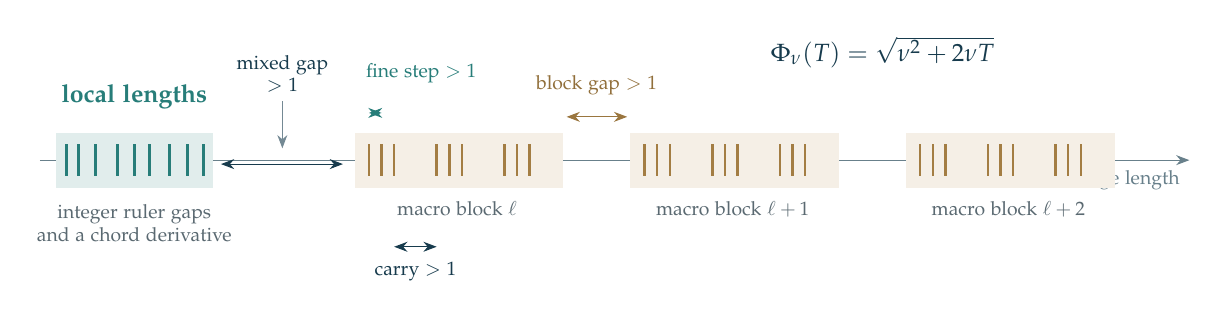
\begin{tikzpicture}[x=1cm,y=1cm,>=Stealth,font=\scriptsize]
\draw[ink!65,->] (0,0)--(14.6,0) node[below left] {edge length};
\fill[teal!14] (.2,-.35) rectangle (2.2,.35);
\foreach \x in {.34,.49,.71,.99,1.2,1.39,1.65,1.88,2.08} \draw[teal,line width=1pt] (\x,-.2)--(\x,.2);
\node[text=teal,font=\small\bfseries,align=center] at (1.2,.8) {local lengths};
\node[text=slate,align=center] at (1.2,-.8) {integer ruler gaps\\and a chord derivative};
\foreach \s/\lab in {4/{\ell},7.5/{\ell+1},11/{\ell+2}}{
\fill[gold!14] (\s,-.35) rectangle ({\s+2.65},.35);
\foreach \i in {0,1,2} {\foreach \j in {0,1,2} {\draw[gold!90!black,line width=.9pt] ({\s+.18+.86*\i+.16*\j},-.2)--++(0,.4);}}
\node[text=slate] at ({\s+1.3},-.62) {macro block $\lab$};}
\draw[<->,ink] (2.3,-.05)--(3.85,-.05);
\node[text=ink,align=center] at (3.08,1.1) {mixed gap\\$>1$};
\draw[->,ink!60] (3.08,.75)--(3.08,.15);
\draw[<->,teal] (4.18,.6)--(4.34,.6);
\node[anchor=south west,text=teal,align=left] at (4.02,.86) {fine step $>1$};
\draw[<->,ink] (4.5,-1.1)--(5.04,-1.1);
\node[below,text=ink] at (4.77,-1.17) {carry $>1$};
\draw[<->,gold!85!black] (6.69,.55)--(7.46,.55);
\node[above,text=gold!80!black,align=center] at (7.07,.7) {block gap $>1$};
\node[text=ink,font=\small\bfseries] at (10.7,1.37) {$\Phi_\nu(T)=\sqrt{\nu^2+2\nu T}$};
\end{tikzpicture}
\caption{The proof accounts for every pair of different edges: two local
edges, a local and a cross edge, or two cross edges. Within a cross block,
lexicographic order reduces the checks to fine steps and carries; between
blocks, the macro baseline pays for the full digit excursion. Schematic,
not to scale.}
\label{fig:spectrum}
\end{figure}


\subsection{The coefficient and the arbitrary-size passage}

We have $\tau>63/64$, $s\le9/8$, $K\le\xi m^2+1$, and
$s^3\le1+4\xi$. Dividing \eqref{eq:epsilon-diameter} by $(mk)^2$ yields
\begin{align*}
 \frac{\diam\{x_{Ai}\}}{(mk)^2}
 &\le(1+4\xi)(1/2+\xi)+3/m^2\\
 &\le1/2+(7/2)\xi+3/m^2\le1/2+4\xi.
\end{align*}
For the last step use $m\ge1024/\xi$, which implies $3/m^2\le\xi/2$.

Put $m_0=\lceil1024/\xi\rceil$. Given $n\ge4m_0$, choose
$k=\lfloor n/m_0\rfloor$ and $m=\lceil n/k\rceil$. Then
$k\ge4$. The inequalities $km_0\le n<(k+1)m_0$ give
$m_0\le m\le m_0+\lceil m_0/k\rceil\le2m_0$, and
\[
 n\le mk<n+k\le(1+1/m_0)n.
\]
Delete points to obtain exactly $n$ and pad coordinates to dimension
$10m_0-1$. Neither operation worsens the required estimates. Since
$1/m_0\le\xi/1024$,
\begin{equation}\label{eq:rounding-bound}
 \diam X<(1/2+4\xi)(1+\xi/1024)^2n^2<(1/2+5\xi)n^2.
\end{equation}
For example, the last inequality follows from $1/2+4\xi\le1$ and
$(1+\xi/1024)^2-1<\xi$. Choosing $\xi=\varepsilon/8$ proves
\cref{thm:epsilon}, with strictly positive coefficient slack.

For \cref{cor:uniform}, choose
$\xi=\max\{20480/d,8192/n\}$. The hypotheses imply $0<\xi\le1/8$.
Moreover $10\lceil1024/\xi\rceil-1\le d$ and
$4\lceil1024/\xi\rceil\le n$: the respective left sides are at most
$d/2+9$ and $n/2+4$. Apply \eqref{eq:rounding-bound}, use
$\max\{u,v\}\le u+v$, and pad to dimension $d$.

\section{Six macro vertices and dimension 29}\label{sec:r29-proof}

The preceding uniform estimates favor a large number of clusters. To
obtain a small fixed dimension, we instead keep $m=6$ and certify the
entire macro completion directly. All parameters are rational:
\begin{equation}\label{eq:r29-parameters}
\begin{gathered}
 K=457/25,\quad H=569/500,\quad\eta=533/500,\quad\sigma=138/125,\\
 a=519/1000,\quad b=879/500,\quad r_0=507/100,\quad r_1=1131/100,\\
 k_0=100,\qquad t=971/1000,\qquad C=101/100.
\end{gathered}
\end{equation}
We work for every integer $k\ge100$ and every prime $p$ such that
\begin{equation}\label{eq:admissible-prime}
 6k<p\le6Ck.
\end{equation}

\subsection{A finite macro certificate}

Use the symmetric label matrix
\begin{equation}\label{eq:labels29}
 \ell=\begin{pmatrix}
 0&3&5&7&14&15\\3&0&2&4&13&12\\5&2&0&1&11&10\\
 7&4&1&0&9&8\\14&13&11&9&0&6\\15&12&10&8&6&0
 \end{pmatrix}.
\end{equation}
Its upper-triangular labels are exactly $1,\ldots,15$. For $A\ne B$, put
$D_{AB}=K+H\ell_{AB}$ and $E_{AB}=D_{AB}^2-2(r_0^2+r_1^2)$; put both
diagonal entries equal to zero. Define the $5\times5$ anchored Gram matrix
\[
 B_{ij}=\frac{E_{0i}+E_{0j}-E_{ij}}2\qquad(1\le i,j\le5).
\]
Let $P^G_{AJ}=D_{AJ}$ for $A<J$ and zero otherwise, and set $P^F=D-P^G$.
For $\star\in\{F,G\}$ define the $5\times6$ matrix
\[
 T^\star_{jA}=P^\star_{A0}-P^\star_{Aj}\qquad(1\le j\le5,\ 0\le A\le5).
\]
The three rational matrices to be checked are
\begin{equation}\label{eq:three-matrices}
 B,\qquad M(x)=B-\frac{(\sigma T^G+\eta xT^F)(\sigma T^G+\eta xT^F)^\T}{(ar_0)^2},
 \quad x\in\{0,1/100\}.
\end{equation}

\begin{lemma}[Exact whole-matrix certificate]\label[lemma]{lem:matrix29}
All three matrices in \eqref{eq:three-matrices} are positive definite.
\end{lemma}
\begin{proof}
Substitute the rational parameters \eqref{eq:r29-parameters} and the
integer matrix \eqref{eq:labels29}, then eliminate successively without
pivoting. Every diagonal pivot in the resulting $LDL^\T$ factorization
is a strictly positive rational. \Cref{tab:pivots} gives certified rational
lower bounds for all fifteen pivots; the exact recurrence and a complete
stand-alone reconstruction program are in \cref{app:certificate}.
No floating-point positivity decision is used.
\end{proof}

\begin{table}[ht]
\centering\small
\begin{tabular}{@{}lccccc@{}}
\toprule
Matrix & $d_1$ & $d_2$ & $d_3$ & $d_4$ & $d_5$\\
\midrule
$B$ & $>1$ & $>1$ & $>1$ & $>1$ & $>1$\\[3pt]
$M(0)$ & $>1$ & $>1$ & $>\frac{1}{2}$ & $>1$ & $>1$\\[3pt]
$M(1/100)$ & $>1$ & $>1$ & $>\frac{1}{2}$ & $>1$ & $>1$\\[3pt]
\bottomrule
\end{tabular}
\caption{Strict rational lower bounds for the five successive $LDL^\T$ pivots of each matrix. These are lower bounds, not rounded pivot values. Every entry is obtained by exact fraction arithmetic.}
\label{tab:pivots}
\end{table}


Choose $q_0=0$ and $q_1,\ldots,q_5\in\R^5$ with Gram matrix $B$. The
polarization identity then gives $\norm{q_A-q_B}^2=E_{AB}$. Let $Q$ be the
square matrix with columns $q_1,\ldots,q_5$ and define
$F=Q^{-\T}T^F$, $G=Q^{-\T}T^G$. Subtracting their anchored inner products
gives
\[
 \ip{q_A-q_J}{F_A}=P^F_{AJ},\qquad
 \ip{q_A-q_J}{G_A}=P^G_{AJ}.
\]
By \cref{lem:matrix29}, both endpoint matrices
$Q^{-\T}(\sigma T^G+\eta xT^F)$ have norm less than $ar_0$.
Indeed, writing $A(x)=\sigma T^G+\eta xT^F$, congruence gives
\[
 Q^{-\T}M(x)Q^{-1}
 =I-\frac{[Q^{-\T}A(x)][Q^{-\T}A(x)]^\T}{(ar_0)^2}\succ0.
\]
The matrix depends affinely on $x$, and the operator norm is convex.
Thus the same strict bound holds for every $x\in[0,1/100]$. In particular,
\begin{equation}\label{eq:finite-k-operator}
 U=\frac{k}{a}(\eta F+\sigma kG)
   =\frac{k^2}{a}Q^{-\T}A(1/k)
 \quad\text{satisfies}\quad \opnorm U<r_0k^2
 \qquad(k\ge100).
\end{equation}
This is why the two endpoint checks control every finite $k\ge100$.

\subsection{Coordinates and cross lengths}

Put $S=k^2$, $R_0=r_0k^2$, $R_1=r_1k^2$, and $\theta=a/k$. Use the same
uniform digit marks $f_i$ as before, and the independent ruler marks
\begin{equation}\label{eq:ruler29}
 y_{Ai}=2pi+[i^2+2kAi]_p,\qquad w_{Ai}=\frac{b\,y_{Ai}}{2pk}.
\end{equation}
With $U$ from \eqref{eq:finite-k-operator}, construct the actual points by
\eqref{eq:points}. Their coordinate blocks have dimensions $5,6,6,6,6$,
so the ambient dimension is exactly~29. The cross identity becomes
\begin{equation}\label{eq:r29-cross}
 \norm{x_{Ai}-x_{Bj}}=\Phi_\nu(\sigma kf_i+\eta f_j),
 \qquad\nu=k^2D_{AB},\quad A<B.
\end{equation}

Let $\gamma=1-a^2/8$ and $T_{\max}=(\sigma k+\eta)(k-1)/2$.
Since $\sigma\ge\eta$, $2T_{\max}<\sigma k^2$. The rational inequalities
\begin{equation}\label{eq:r29-cross-guards}
\begin{gathered}
 t^2<1-\frac{\sigma}{K+H},\quad t\eta\gamma>1,\quad
 \sigma\gamma-\eta>0,\quad t\eta>1,\\
 H-\sigma/t>0,\quad\sigma-\eta>0,\quad\eta/t>1
\end{gathered}
\end{equation}
imply $t\le\Phi_\nu'(T)\le1/t$ on every digit interval. They are verified
by direct rational substitution in the certificate accompanying
\cref{lem:matrix29}.

Fine steps have length gap at least $t\eta\gamma>1$. Carries have digit
increment at least $(\sigma\gamma-\eta)k+\eta$, giving a length gap
greater than one. Successive macro labels differ by one, so their
baseline gap is $Hk^2$, and the separation between blocks is at least
\[
 Hk^2-2T_{\max}/t
 =(H-\sigma/t)k^2+(\sigma-\eta)k/t+\eta/t>1.
\]
Thus all cross-edge lengths are mutually strictly separated.

\subsection{Local lengths and the mixed gap}

For a local edge, write $d=j-i$ and $g=y_{Aj}-y_{Ai}$. Then
\[
 (2d-1)p<g<(2d+1)p,\qquad g\equiv d(2i+d+2kA)\pmod p.
\]
By \cref{lem:residue-ruler}, now with $m=6$ and $L=2$, all these
differences are distinct positive integers and their lags are nondecreasing
in $g$.

The local lengths are now
\[
 L(d,g)=\sqrt{H_d^2+B(g)^2},\quad
 H_d=2R_0\sin\frac{ad}{2k},\quad B(g)=2R_1\sin\frac{bg}{4pk}.
\]
Both factors increase over their relevant ranges. In comparing two
ordered ruler differences, keep the smaller lag $d_1$ fixed. Since
$g\ge pd_1$ and the angle in $B$ lies in $(0,b/2)$, sine concavity gives
\[
 B(g)\ge r_1k\sin(b/2)d_1,\qquad
 B'(g)\ge\frac{r_1b\cos(b/2)}{12C},\qquad
 H_{d_1}\le r_0akd_1.
\]
It follows that
\begin{equation}\label{eq:local-derivative29}
 \frac{\partial L(d_1,g)}{\partial g}\ge
 \frac{r_1b\cos(b/2)/(12C)}
 {\sqrt{1+[r_0a/(r_1\sin(b/2))]^2}}>1.
\end{equation}
The last inequality is an exact rational consequence of the alternating
Taylor bounds, with $z=b/2\in(0,1)$,
\[
 z-z^3/6\le\sin z\le z-z^3/6+z^5/120,\qquad
 \cos z\ge1-z^2/2+z^4/24-z^6/720.
\]
The square of the lower bound in \eqref{eq:local-derivative29} exceeds
one by a strictly positive rational, checked in the same certificate.
Apply \cref{lem:local-comparison} with
$c=r_0a/[r_1\sin(b/2)]$ and $v=r_1b\cos(b/2)/(12C)$.
The integer gap in $g$ proves strict separation of all local lengths.

The minimum local distance is at least $r_1k\sin(b/2)>1$. Using the same
Taylor upper bound and $\sin u\le u$, every local length is less than
$18k^2$. For cross lengths, $2|T|/\nu<\sigma/(K+H)<1-t^2$ gives
$\Phi_\nu(T)>t\nu\ge t(K+H)k^2>(37/2)k^2$.
Thus the mixed gap is greater than $k^2/2>1$.
All pair distances are positive, so the indexing is injective.

\subsection{Diameter and the prime-first sizes}

The cross lengths, and hence all lengths, are less than
\[
 [K+15H+\sigma/(2t)]k^2.
\]
For $n=6k$, the corresponding coefficient is
\begin{equation}\label{eq:diameter29}
 \frac{K+15H+\sigma/(2t)}{36}
 =\frac{697537}{699120}<\frac{499}{500}.
\end{equation}
The diameter is the largest of these finitely many edge lengths.

For every sufficiently large prime $p$, let $k=\lfloor(p-1)/6\rfloor$.
Then $6k<p\le6(k+1)\le6Ck$ whenever $k\ge100$. Infinitude of primes gives
unbounded such $k$. Choosing a large enough prime makes $6k\ge N$ and
proves \cref{thm:r29}. No prime number theorem or short-interval prime
estimate is required for this theorem.

\subsection{Every sufficiently large size}

To prove \cref{cor:r29-all}, set $k=\lceil n/6\rceil$ and $x=6k$.
Dusart's explicit bound \cite[Proposition~6.8]{Dusart} supplies a prime
\[
 x<p\le x\left(1+\frac{1}{25(\log x)^2}\right)
 \quad(x\ge396738).
\]
Here $x\ge n\ge400000$ and $\log x>2$, so $6k<p<1.01(6k)$.
Thus \eqref{eq:admissible-prime} holds and $k\ge100$. The preceding
construction gives $6k$ points, with strict edge-length separation and
diameter $<0.998(6k)^2$. Delete points until exactly $n$ remain.
All separation properties persist and the diameter cannot increase.
Since $6k\le n+5$ and
\[
 \frac{999}{1000}
 -\frac{499}{500}\left(1+\frac{5}{400000}\right)^2
 =\frac{3120159501}{3200000000000}>0,
\]
the diameter is $<0.999n^2$. This use of Dusart's unconditional theorem
is a literature input, not a new proof or formal verification of the
prime-interval bound. The threshold is deliberately conservative.

\section{Formalization and provenance}\label{sec:formal}

The two-circle family, its uniform form, and the prime-first dimension-29
theorem have corresponding Lean~4 declarations, listed in
\cref{tab:lean}. Both newer developments use Lean~4.33.1 and the same locked
Mathlib revision; the exact source identities are in \cref{app:sources}.
The recorded final transitive axiom reports contain only
\code{propext}, \code{Classical.choice}, and \code{Quot.sound}.
The epsilon-family endpoints have only the numerical hypotheses of
\cref{thm:epsilon,cor:uniform}; the geometric and operator estimates are
proved within the development.

\begin{table}[ht]
\centering\footnotesize
\begin{tabularx}{\textwidth}{@{}p{.25\textwidth}X@{}}
\toprule
Mathematical conclusion & Exact Lean declaration\\\midrule
Two-circle family & \code{Erdos670EpsilonFamily.epsilon\_family}\\[3pt]
Uniform dimension bound & \code{Erdos670EpsilonFamily.uniform\_family}\\[3pt]
R29 indexed configuration & \code{Erdos670R29.r29\_unbounded\_counterexamples}\\[3pt]
R29 finite-set statement & \code{Erdos670R29Minimal.finite\_set\_counterexamples}\\[3pt]
R29 conjecture negation & \code{Erdos670R29Minimal.not\_fixedDimensionStatement\_r29}\\
\bottomrule
\end{tabularx}
\caption{The exact endpoint names. The finite-set translation and the indexed
geometric theorem are distinct declarations.}
\label{tab:lean}
\end{table}

The indexed R29 theorem and its finite-set adapter have different roles:
the first constructs the points, and the second transports that result to
the fixed-dimensional proposition \eqref{eq:conjecture}. The adapter uses
the exact statement extracted from the pinned Formal Conjectures source.
Its unit edge-separation inequality is weak, as in \cref{thm:r29}, although
the written estimates above give strict separation. The earlier public
$\R^{81794}$ theorem has a separate proof and statement adapter
\cite{PublishedFinite,PublicStatus}.

The existing epsilon-family compilation reused checked imports. The R29
records additionally include a build from zero local project objects with
pinned upstream caches and a later reported fresh official-kernel replay.
These are source-specific execution records; preparing this exposition
has not performed a new Lean build. The public repository preserves the
statements and audit receipts, rather than the complete newer Lean proof
closures. Those closures remain private. Formal checking and the
arithmetic certificate in \cref{app:certificate} do not constitute
independent human proof or priority review.

The quadratic-residue ruler is classical in the Erd\H{o}s--Tur\'an
tradition \cite{ErdosTuran}. Euclidean Gram realization,
positive-semidefinite completion, and weighted Schur estimates are also
classical \cite{Schoenberg,Schur,Sinnamon,Robinson}. Orthogonal-circle
geometry has classical precedents in Lenz-type constructions
\cite{ErdosLenz}. The colex macro estimates are inherited from the earlier
manuscript. Here the digit and ruler circles are separated, and the
small-dimensional construction uses the finite non-colex seed
\eqref{eq:labels29}.

This research and manuscript were developed with substantial AI assistance
in mathematical exploration, proof engineering, source comparison, and
writing. An AI-generated simplification and readability rewrite informed
the earlier orthogonal-circle construction, with permission to use it.
Independent mathematical review remains open. The earlier Palomar and
Prove2Me records concern only the archived $0.74$ theorem
\cite{PublicStatus}.

\section{What remains open}\label{sec:open}

The coefficient-one fixed-dimensional proposition is refuted by a single
fixed dimension. Its failure does not determine the exact asymptotic
diameter in each dimension. Three concrete questions remain:
\begin{enumerate}[leftmargin=1.7em,itemsep=4pt]
\item Does the coefficient-one bound fail in the plane, or in another
 prescribed dimension below~29?
\item Can one fixed dimension support genuine unit-separated edge lengths
 with diameter $(1/2+o(1))n^2$? The dimension-dependent tolerance family does
 not answer this question.
\item What is the best tradeoff between dimension, the all-size threshold,
 and the diameter coefficient? The finite macro certificate and uniform
 colex estimates optimize different aspects of that tradeoff.
\end{enumerate}
No lower bound on the dimension required by an arbitrary construction is
claimed here. Nor do the displayed constants establish optimality within
all two-circle constructions.

\section*{Acknowledgments}
The author thanks Boon Suan Ho for helpful comments on an earlier draft of this manuscript.


\appendix
\section{Proof of the macro input}\label{app:macro}

We prove \cref{lem:macro}, following the first version's macro
estimates~\cite[Lemmas~2--3]{Tripodo}. None of the cluster geometry of
the main text is used here. The plan is as follows.
\begin{enumerate}[leftmargin=2em,itemsep=1pt]
\item Compute the Gram matrix $\Gamma$ of the \emph{increments}
 $q_j-q_{j-1}$ that the colex distances would require
 (\cref{sec:app-gram}).
\item Show that $\Gamma$ is dominated by its tridiagonal part, and that
 this part contains two ``reserves'' of positivity: one large
 enough to pay for the shortening by $2\rho^2$, and one diagonal reserve
 (\cref{sec:app-reserves}). This proves the Euclidean realization.
\item Use the diagonal reserve to bound the vectors $F_A,G_A$ all at once,
 through their projections on the increments (\cref{sec:app-projections}).
 This proves the whole-matrix estimates.
\end{enumerate}
Throughout, $m\ge4$ and $K,\rho$ satisfy \eqref{eq:macro-gates}. Since
$H_m\ge1$, the harmonic gate implies $K\ge16384>10$, as used below. Vectors
$x\in\R^{m-1}$ are indexed $x_1,\dots,x_{m-1}$, and $e_A$ $(0\le A<m)$
denotes the standard basis of $\R^m$.

\subsection{The increment Gram matrix}\label{sec:app-gram}

Let $\partial$ be the $(m-1)\times m$ matrix whose $j$-th row is
$e_{j-1}^\T-e_j^\T$ $(1\le j<m)$. For a symmetric $m\times m$ matrix
$\mathbf D$ with zero diagonal, the matrix $-\frac12\partial\mathbf
D\partial^\T$ is the Gram matrix that the increments must have: if points
$q_A$ satisfy $\norm{q_A-q_B}^2=\mathbf D_{AB}$, then
$\ip{q_i-q_{i-1}}{q_j-q_{j-1}}=(-\frac12\partial\mathbf D\partial^\T)_{ij}$,
by the polarization identity. This is Schoenberg's Euclidean-distance
criterion in consecutive-increment coordinates~\cite[Theorem~1]{Schoenberg}.

Let $\mathbf D$ have entries $D_{AB}^2$ off the diagonal, put
$\Gamma=-\frac12\partial\mathbf D\partial^\T$, and write
\[
 D_j=D_{j-1,j}=K+\frac{j(j+1)}2\qquad(1\le j<m)
\]
for the lengths of the consecutive macro edges. Since
$D_{j-1,j+1}=D_j+j$ and $D_{j,j+1}=D_j+j+1$, a direct computation gives
\begin{equation}\label{eq:gram-entries}
 \Gamma_{jj}=D_j^2,\qquad
 \Gamma_{j,j+1}=-c_j,\quad\text{where }\ c_j=\tfrac12(D_j+1)^2+j.
\end{equation}
If $i\le j-2$, the four lengths $D_{i-1,j-1},D_{i-1,j},D_{i,j-1},D_{ij}$ have
the form $\alpha,\beta,\alpha+1,\beta+1$ with $\beta-\alpha=j-1$, and
therefore $\Gamma_{ij}=-(j-1)$. In other words, $\Gamma_{ij}=-(\max\{i,j\}-1)$
whenever $|i-j|\ge2$.

\subsection{Two reserves of positivity}\label{sec:app-reserves}

Split $\Gamma=\mathsf B-\mathsf N$, where the \emph{band} $\mathsf B$
keeps the diagonal and the two neighbouring diagonals of $\Gamma$, and the
\emph{far part} $\mathsf N$ has entries $\max\{i,j\}-1$ for $|i-j|\ge2$
and zero otherwise. Completing squares in $-2c_jx_jx_{j+1}$ gives
\begin{equation}\label{eq:tridiagonal}
 \mathsf B[x]=\sum_{j=1}^{m-2}c_j(x_j-x_{j+1})^2
              +\sum_{j=1}^{m-1}\alpha_jx_j^2+c_{m-1}x_{m-1}^2,
\end{equation}
where $c_{m-1}$ is given by the same formula as the other $c_j$,
$\alpha_j=D_j^2-c_j-c_{j-1}$ with $c_0=0$, and explicitly
\[
 \alpha_1=\frac{K^2}2-2,\qquad \alpha_2=-4,\qquad
 \alpha_j=(j-2)K+\frac{j^3}2-j^2-2j\quad(j\ge3).
\]

\emph{The band dominates a diagonal form.} Define
$\Omega=\diag(\omega_1,\dots,\omega_{m-1})$ by
\[
 \omega_1=\omega_2=\frac{K^2}{24},\qquad \omega_j=\frac{Kj+j^3}{24}\quad(j\ge3).
\]
We claim $\mathsf B\succeq\Omega$. The terms of \eqref{eq:tridiagonal}
involving only $x_1,x_2$ are $c_1(u-v)^2+\alpha_1u^2-4v^2$, with
$u=x_1$, $v=x_2$. Since $c_1,\alpha_1\ge K^2/4$ and
$(u-v)^2+u^2\ge(u^2+v^2)/3$,
\[
 c_1(u-v)^2+\alpha_1u^2-4v^2
 \ge\frac{K^2}{12}(u^2+v^2)-4v^2
 \ge\frac{K^2}{24}(u^2+v^2)
\]
for $K\ge10$. For $j\ge3$ we have $\alpha_j\ge\omega_j$, because
\[
 24(\alpha_j-\omega_j)=(23j-48)K+11j^3-24j^2-48j,
\]
which is positive at $j=3$ (it equals $21K-63$), and has both terms
nonnegative for $j\ge4$. All remaining terms of \eqref{eq:tridiagonal}
are nonnegative.

\emph{The far part is small.} Put $\sigma_0=\sum_j\omega_j^{-1}$ and
$\sigma_2=\sum_jj^2\omega_j^{-1}$. For $K\ge10$,
\[
 \sigma_0\le\frac{48}{K^2}+\frac{24H_m}{K}\le\frac{29H_m}{K},
 \qquad
 \sigma_2\le\frac{120}{K^2}+24H_m\le26H_m.
\]
With $b_0=\sum_j|x_j|$ and $b_1=\sum_jj|x_j|$ we have
$|\mathsf N[x]|\le\sum_{i,j}\max\{i,j\}|x_i||x_j|\le2b_0b_1$, while
weighted Cauchy--Schwarz gives $b_0^2\le\sigma_0\Omega[x]$ and
$b_1^2\le\sigma_2\Omega[x]$. Therefore
\begin{equation}\label{eq:remainder}
 |\mathsf N[x]|
 \le2\sqrt{\sigma_0\sigma_2}\,\Omega[x]
 \le\frac{\sqrt{754}}{64}\,\Omega[x]
 \le\tfrac12\Omega[x]\le\tfrac12\mathsf B[x],
\end{equation}
using $K\ge16384H_m^2$ (so that $\sqrt{29\cdot26}\,H_m/\sqrt K\le\sqrt{754}/128$)
and $754<1024$. Hence
\[
 \Gamma\succeq\tfrac12\mathsf B.
\]

\emph{First reserve: a path energy.} Let $\Pi$ be the quadratic form
\[
 \Pi[x]=D_1^2x_1^2+\sum_{j=1}^{m-2}D_j^2(x_j-x_{j+1})^2+D_{m-1}^2x_{m-1}^2.
\]
In \eqref{eq:tridiagonal}, bound $-4x_2^2\ge-8x_1^2-8(x_2-x_1)^2$. Since
$\alpha_1-8\ge D_1^2/4$, $c_1-8\ge D_1^2/4$, $c_j\ge D_j^2/4$ for all $j$,
and $\alpha_j\ge0$ for $j\ge3$, this proves
\begin{equation}\label{eq:path-reserve}
 \mathsf B\succeq\tfrac14\Pi.
\end{equation}

\emph{Second reserve: a diagonal.} For every $j$,
\begin{equation}\label{eq:diagonal-reserve}
 D_j^2\le36(K+m)\,\omega_j,
 \qquad\text{hence}\qquad
 \mathsf B\succeq\Omega\succeq\frac{\diag(D_1^2,\ldots,D_{m-1}^2)}{36(K+m)}.
\end{equation}
For $j=1,2$ the first inequality is immediate. For $j\ge3$, use
$D_j\le K+j^2\le(K+m)j$ to get the stronger bound
$D_j^2\le(K+j^2)(K+m)j=(K+m)(Kj+j^3)$.

\emph{Paying for the shortening.} Shortening every squared distance by
$2\rho^2$ replaces $\mathbf D$ by $\mathbf D_\rho$, with entries
$D_{AB}^2-2\rho^2$ off the diagonal. Since the rows of $\partial$ sum to
zero, the new increment Gram matrix is
\[
 \Gamma_\rho=-\tfrac12\partial\mathbf D_\rho\partial^\T
 =\Gamma-\rho^2\partial\partial^\T.
\]
Now $\partial\partial^\T[x]=x_1^2+\sum_j(x_j-x_{j+1})^2+x_{m-1}^2\le
\Pi[x]/K^2$, because every $D_j\ge K$. As $\rho\le K/4$, the subtraction
costs at most $\Pi/16\preceq\mathsf B/4$, by \eqref{eq:path-reserve}.
Combining this with $\Gamma\succeq\mathsf B/2$ and the two reserves,
\begin{equation}\label{eq:both-reserves}
 \Gamma_\rho\succeq\tfrac14\mathsf B\succeq\tfrac1{16}\Pi\succ0,
 \qquad
 \Gamma_\rho\succeq
     \frac{\diag(D_1^2,\ldots,D_{m-1}^2)}{144(K+m)}.
\end{equation}
Here $\Pi\succ0$ because $\Pi\succeq K^2\partial\partial^\T$ and $\partial$
has full row rank.

\emph{Euclidean realization.} Since $\Gamma_\rho\succ0$, we may write
$\Gamma_\rho=\mathsf V^\T\mathsf V$ for an invertible
$(m-1)\times(m-1)$ matrix $\mathsf V$ with columns $v_1,\dots,v_{m-1}$
(for instance, by Cholesky factorization). Put $q_0=0$ and
$q_A=v_1+\dots+v_A$. For $A<B$ let $u_{AB}=\sum_{j=A+1}^Be_j\in\R^{m-1}$;
then $\partial^\T u_{AB}=e_A-e_B$, and so
\[
 \norm{q_B-q_A}^2
 =\Gamma_\rho[u_{AB}]
 =-\tfrac12(e_A-e_B)^\T\mathbf D_\rho(e_A-e_B)
 =D_{AB}^2-2\rho^2.
\]
The increments $v_j=q_j-q_{j-1}$ are linearly independent, so the points
$q_A$ are affinely independent.

\subsection{Bounding all projections at once}\label{sec:app-projections}

Let $Y_0,\dots,Y_{m-1}\in\R^{m-1}$ be vectors, and record their
projections on the increments in the $(m-1)\times m$ matrix
\[
 Z_{jA}=\ip{q_j-q_{j-1}}{Y_A},\qquad\text{that is,}\qquad Z=\mathsf V^\T Y.
\]
As $\mathsf V$ is invertible, $Z$ determines $Y$, and
$Y^\T Y=Z^\T(\mathsf V^\T\mathsf V)^{-1}Z=Z^\T\Gamma_\rho^{-1}Z$. Writing
$\mathsf P=\diag(D_1,\dots,D_{m-1})$, the second inequality in
\eqref{eq:both-reserves} gives
$\Gamma_\rho^{-1}\preceq144(K+m)\mathsf P^{-2}$, and hence
\begin{equation}\label{eq:whole-solve}
 \opnorm Y\le12\sqrt{K+m}\,\opnorm{\mathsf P^{-1}Z}.
\end{equation}
So it suffices to show that the projection matrices of $F$ and $G$,
normalized by $\mathsf P^{-1}$, have bounded operator norm.

Taking consecutive differences of the defining equations
\eqref{eq:anchored-projections} (with the convention that the right-hand
sides vanish for $J=A$) gives, for $1\le j<m$ and $0\le A<m$,
\begin{align*}
 Z^F_{jA}&=D_j\,\one_{A=j}-\one_{A>j},\\
 Z^G_{jA}&=-D_j\,\one_{A=j-1}-(j-1)\,\one_{A<j-1}.
\end{align*}
For example, for $A>j$ we get $Z^F_{jA}=D_{j-1,A}-D_{jA}=-1$, because the
colex labels of $\{j-1,A\}$ and $\{j,A\}$ differ by one. The columns $F_0$
and $G_{m-1}$ vanish. Delete them, and index the remaining columns by
$1,\dots,m-1$ (column $A$ of $Z^F$, and column $A-1$ of $Z^G$, become
column $A$). The two projection matrices become
\[
 Z_{\mathrm{fine}}=\mathsf P-\mathsf E_+,\qquad
 Z_{\mathrm{coarse}}=-(\mathsf P+\mathsf E_-),
\]
where $(\mathsf E_+)_{ij}=\one_{i<j}$ and
$(\mathsf E_-)_{ij}=(i-1)\one_{j<i}$.

For the first matrix, the Frobenius norm gives
$\opnorm{\mathsf P^{-1}\mathsf E_+}\le m/K\le1$, as all entries of
$\mathsf P^{-1}\mathsf E_+$ are at most $1/K$. For the second,
\[
 0\le(\mathsf P^{-1}\mathsf E_-)_{ij}
 =\frac{i-1}{D_i}\one_{j<i}
 \le\frac2i\one_{j<i}
\]
since $D_i\ge i(i+1)/2$. The finite Hardy matrix
$\mathcal H_{ij}=i^{-1}\one_{j<i}$ has operator norm at most $2$ by the
weighted Schur test~\cite{Schur,Sinnamon}. For completeness, take
the weights $w_j=j^{-1/2}$; by comparison with integrals,
\[
 \sum_{j<i}\frac{w_j}{i}\le2w_i,
 \qquad \sum_{i>j}\frac{w_i}{i}\le2w_j.
\]
For any real vector $x$, Cauchy--Schwarz with these weights then gives
\[
 \sum_i\Bigl(\sum_j \mathcal H_{ij}x_j\Bigr)^2
 \le\sum_i\Bigl(\sum_j\mathcal H_{ij}w_j\Bigr)
          \Bigl(\sum_j\mathcal H_{ij}\frac{x_j^2}{w_j}\Bigr)
 \le\sum_j\frac{x_j^2}{w_j}\sum_i2w_i\mathcal H_{ij}
 \le4\sum_jx_j^2.
\]
A matrix with nonnegative entries bounded by those of $2\mathcal H$ has
operator norm at most $2\opnorm{\mathcal H}$ (apply it to $|x|$), so
$\opnorm{\mathsf P^{-1}\mathsf E_-}\le4$.

Thus $\opnorm{\mathsf P^{-1}Z_{\mathrm{fine}}}\le2$ and
$\opnorm{\mathsf P^{-1}Z_{\mathrm{coarse}}}\le5$, and
\eqref{eq:whole-solve} gives $\opnorm F\le24\sqrt{K+m}$ and
$\opnorm G\le60\sqrt{K+m}$; restoring the zero columns does not change
the norms. This proves \eqref{eq:FG} and completes the proof of
\cref{lem:macro}.
\qed




\section{Reconstructing the rational certificate}\label{app:certificate}
The matrices in \eqref{eq:three-matrices} are determined entirely by the
displayed rational parameters and label matrix. Starting with a symmetric
matrix $A^{(0)}$, successive elimination uses
\[
 d_k=A^{(k-1)}_{kk},\qquad
 A^{(k)}_{ij}=A^{(k-1)}_{ij}
 -\frac{A^{(k-1)}_{ik}A^{(k-1)}_{jk}}{d_k}\quad(i,j>k).
\]
If every $d_k$ is positive, this is an $LDL^\T$ decomposition with positive
diagonal, so the matrix is positive definite. All inputs and operations
are rational. The following complete Python program reconstructs all
three matrices, checks the fifteen positive pivots and the scalar guards,
and prints exact fractions and the lower bounds in \cref{tab:pivots}.
It uses only the Python standard library; checks are not removable
\texttt{assert} statements. Running under \texttt{python3 -O} gives the
same output. No finite sampling in $k$ or floating-point estimate enters
this certificate. The passage to every $k\ge100$ is the operator-norm
convexity argument in \eqref{eq:finite-k-operator}.
\lstinputlisting[language=Python]{certificate_reconstruction.py}


\section{Source correspondence}\label{app:sources}

The written arguments and the formal endpoint sources have different roles.
The prose proofs in \cref{sec:epsilon-proof,sec:r29-proof} reorganize the
retained written construction notes; \cref{sec:formal} identifies the exact
Lean conclusions. In particular, the R29 paper theorem uses the weak unit
edge-separation inequality of the formal statement, although the written
scalar estimates are strict.

\begin{table}[ht]
\centering\footnotesize
\begin{tabularx}{\textwidth}{@{}p{.28\textwidth}X@{}}
\toprule
Source object & Immutable Git blob identity\\\midrule
Two-circle written proof & \texttt{63fdaf3adb4357e39781a9020d8815a4d0de4dca}\\[3pt]
Epsilon-family formal source & \texttt{0670e6c3af874912519aacaa79dd6a9b77f16e22}\\[3pt]
R29 indexed formal source & \texttt{8d09609eef219795b3dce076f3dc10c50a901ee0}\\[3pt]
R29 minimal exact adapter & \texttt{8ac23307f1491887b81d8a6edf67e80a709929fb}\\[3pt]
R29 exact matrix inputs & \texttt{0eea70459e28e7d23ea73f22edf202f37d6eea5c}\\
\bottomrule
\end{tabularx}
\caption{Selected exact source identities, retained for version matching.
A blob identity identifies source bytes; it is not an execution receipt.}
\end{table}

The locked Mathlib revision for the newer endpoints is
\begin{center}\small\texttt{0df444a360eaa60ab8c11dca51a86af692955474}.\end{center}
The extracted Formal Conjectures statement is pinned at project revision
\begin{center}\small\texttt{c77fdd446d23539302aa73bcfae4a9fa962b8382}.\end{center}
Its source blob is \texttt{1ae473043edcd960c0b9eed81ccd6e82994f2a22}.
The public repository preserves statement headers, audit output and build
receipts separately from the paper source. These identities make the
correspondence inspectable; they do not assert that this new typeset
exposition has itself received independent proof or priority review.

\clearpage
\begin{thebibliography}{12}
\raggedright


\bibitem{Erdos}
P.~Erd\H{o}s,
\emph{Some unsolved problems},
in \emph{Combinatorics, Geometry and Probability: A Tribute to Paul Erd\H{o}s},
B.~Bollob\'as and A.~Thomason (eds.),
Cambridge University Press, 1997, pp.~1--10, Problem~20.
\href{https://doi.org/10.1017/CBO9780511662034.004}{doi:10.1017/CBO9780511662034.004}.

\bibitem{ErdosTuran}
P.~Erd\H{o}s and P.~Tur\'an,
\emph{On a problem of Sidon in additive number theory, and on some related problems},
J. London Math. Soc. \textbf{16} (1941), 212--215.
\href{https://doi.org/10.1112/jlms/s1-16.4.212}{doi:10.1112/jlms/s1-16.4.212}.

\bibitem{Ho}
Boon Suan Ho,
\emph{Erd\H{o}s's diameter conjecture for separated distances fails in high dimensions},
2026, \href{https://arxiv.org/abs/2604.15305v1}{arXiv:2604.15305v1}.

\bibitem{Tripodo}
J.~Tripodo,
\emph{Separated Euclidean distances with diameter below $0.74n^2$ in a fixed dimension},
research manuscript, 12 October 2026.
Public source snapshot \TripodoCommit,
\href{https://github.com/jjtripodo-lgtm/erdos-670-fixed-dimension/tree/1e73a12ff1076dd11affadbf619ddbbef587133e}{\texttt{jjtripodo-lgtm/erdos-670-fixed-dimension}},
\texttt{paper/fixed\_dimension\_670.tex}.

\bibitem{Schoenberg}
I.~J. Schoenberg,
\emph{Remarks to Maurice Fr\'echet's article ``Sur la d\'efinition axiomatique d'une classe d'espace distanci\'es vectoriellement applicable sur l'espace de Hilbert''},
Ann. of Math. (2) \textbf{36} (1935), 724--732.
\href{https://doi.org/10.2307/1968654}{doi:10.2307/1968654}.

\bibitem{Schur}
I.~Schur,
\emph{Bemerkungen zur Theorie der beschr\"ankten Bilinearformen mit unendlich vielen Ver\"anderlichen},
J. Reine Angew. Math. \textbf{140} (1911), 1--28.
\href{https://doi.org/10.1515/crll.1911.140.1}{doi:10.1515/crll.1911.140.1}.

\bibitem{Sinnamon}
G.~Sinnamon,
\emph{Schur's lemma and best constants in weighted norm inequalities},
Le Matematiche \textbf{57} (2002), fasc.~II, 185--204.
\url{https://lematematiche.dmi.unict.it/index.php/lematematiche/article/view/207}.

\bibitem{Robinson}
P.~L. Robinson,
\emph{Julia operators and Halmos dilations}, arXiv:1803.09329v1, 2018.
\url{https://arxiv.org/abs/1803.09329v1}.

\bibitem{ErdosLenz}
P.~Erd\H{o}s,
\emph{On sets of distances of $n$ points in Euclidean space},
Publ. Math. Inst. Hungar. Acad. Sci. \textbf{5} (1960), 165--169.
\url{https://users.renyi.hu/~p_erdos/1960-08.pdf}.


\bibitem{PublishedFinite}
J.~Tripodo, \emph{Orthogonal circles and a fixed-dimensional
separated-distance counterexample}, Hexagon preprint
\href{https://hexagonmath.org/2610.00254?version=1}{hexagon:2610.00254v1},
15 October 2026.

\bibitem{GrowingDimension}
J.~Tripodo, \emph{Consecutive Euclidean distances within
square-root-logarithmic excess of the counting bound}, research manuscript, 2026. This is the separate unrestricted-dimensional
result; its source identity is recorded in the companion source map.

\bibitem{IncidenceNote}
J.~Tripodo, \emph{Deterministic all-positive incidence signs},
internal research addendum, 11 October 2026.
Preserved source identity: \texttt{fc556ffdd922ee4183c971ad644f1d1ea3903785}.
This earlier internal source is cited to distinguish the existing asymptotic
order from the later two-circle proof organization; it is not a public deposit.

\bibitem{PublicStatus}
J.~Tripodo, \emph{Erd\H{o}s \#670: result and formalization status},
19 October 2026, immutable documentation snapshot
\href{https://github.com/jjtripodo-lgtm/erdos-670-fixed-dimension/blob/2caf66c312c5d498d17e1c150588684b66300e68/PUBLIC_STATUS.md}{\texttt{2caf66c}}.

\bibitem{Dusart}
P.~Dusart, \emph{Estimates of some functions over primes without R.H.},
\href{https://arxiv.org/abs/1002.0442v1}{arXiv:1002.0442v1}, 2010,
Proposition~6.8, p.~8.

\end{thebibliography}


\end{document}
